\documentclass[../report.tex]{subfiles}

\begin{document}
\begin{figure}[H]
\centering
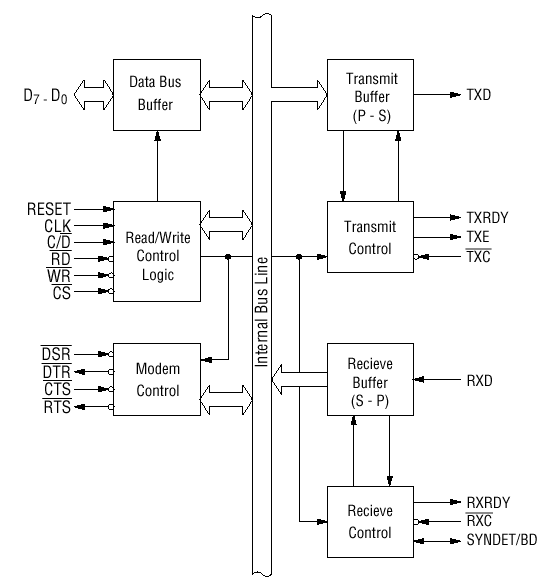
\includegraphics[width=10cm]{figures/8251-usart-architecture.png}
\caption{Kiến trúc của 8251}
\end{figure}

\subsection{Các chân của 8251}
\begin{figure}[H]
\centering
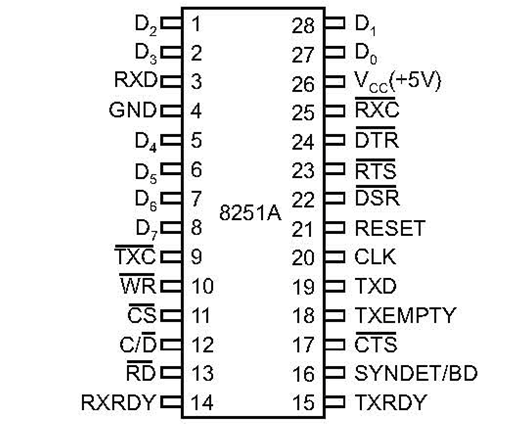
\includegraphics[width=10cm]{figures/8251-usart-pins.png}
\caption{Các chân của 8251}
\end{figure}

\begin{itemize}
\item CLK: Chân nối tới xung đồng hồ của hệ thống. 
\item TxRDY: Tín hiệu báo bộ đềm giữ rỗng (sẵn sàng nhận dữ liệu mới từ CPU). 
\item RxRDY: Tín hiệu báo bộ đệm thu đầy (có kí tự nằm chờ CPU đọc vào). 
\item TxEMPTY: Báo cả đệm giữ và đệm thu đều rỗng. 
\item C/D: CPU chọn thanh ghi lệnh hay thanh ghi dữ liệu. 
\item RxC và TxC: Xung đồng hồ cung cấp cho thanh ghi dịch của phần thu và phát. 
\item RxD và TxD: Nhận và gửi tín hiệu nối tiếp. 
\item D0-D7: Nối với bus dữ liệu của hệ thống. 
\end{itemize}

\subsection{Chế độ được sử dụng}
Trong bài này ta sử dụng 2 giá trị của thanh ghi chế độ và thanh ghi lệnh lần lượt là 01001101b và 00000111b. 
Tương ứng: \\

\begin{figure}[H]
\centering
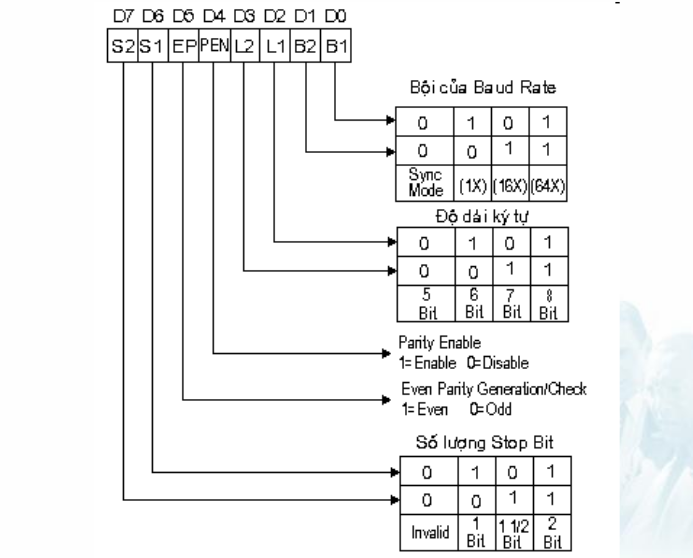
\includegraphics[width=10cm]{figures/8251-che-do.png}
\end{figure}

\noindent Thanh ghi chế độ:
\begin{itemize}
\item Bội của Baurd Rate: 1x.
\item Độ dài kí tự: 8 bit. 
\item Parity: Disable. 
\item Even Parity Generation/Check: Odd. 
\item Số lượng Stop Bit: 1 bit. 
\end{itemize}

\begin{figure}[H]
\centering
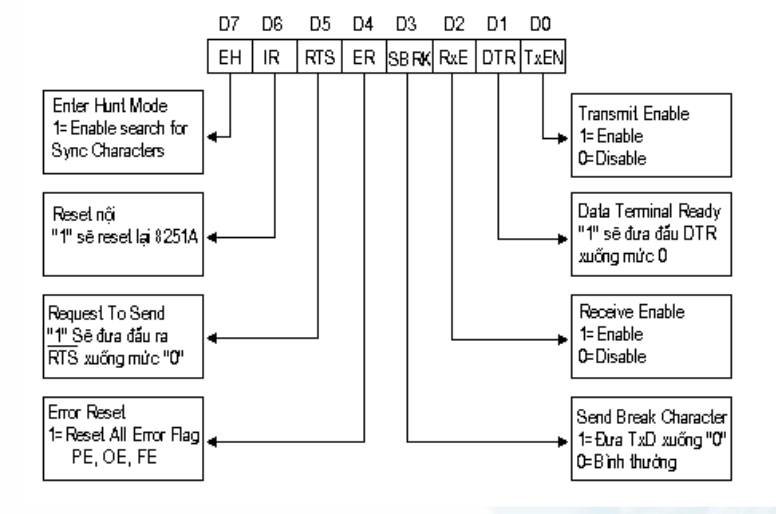
\includegraphics[width=12cm]{figures/8251-lenh.png}
\end{figure}

\noindent Thanh ghi lệnh: 
\begin{itemize}
\item Transmit Enable: Enable. 
\item Data Terminal Ready: 1. 
\item Receive Enable: Enable. 
\item Send Break Character: Bình thường. 
\item Error Restet: Disable. 
\item Request To Send: 0. 
\item Reset nội: 0. 
\item Enter Hunt Mode: Disable. 
\end{itemize}

\subsection{Các bước ghi dữ liệu}
\begin{enumerate}
    \item Đọc 1 byte từ thanh ghi trạng thái vào AL.  
    \item And giá trị nhận được với 0x1. 
    \item Nếu giá trị thu được bằng 0, quay lại bước 1. 
    \item Gán giá trị cần gửi vào AL và ghi ra thanh ghi đệm phát của 8251. 
\end{enumerate}

\subsection{Các bước đọc dữ liệu}
\begin{enumerate}
    \item Đọc 1 byte từ thanh ghi trạng thái vào AL.  
    \item And giá trị nhận được với 0x2. 
    \item Nếu giá trị thu được bằng 0, quay lại bước 1. 
    \item Đọc giá trị từ thanh ghi đệm phát của 8251 vào AL. 
\end{enumerate}

\end{document}
